\subsection{Advanced Techniques}
Kolmogorov-Arnold networks can employ several advanced techniques to simplify the computation of the entire network reducing the time and space complexities. The main techniques are sparsification, pruning, and symbolification \cite{KAN}. 

Figure~\ref{fig:advanced} presents an example of advanced techniques (sparsification, prunig, and Symbolification).

\begin{figure}[H]
    \centering
    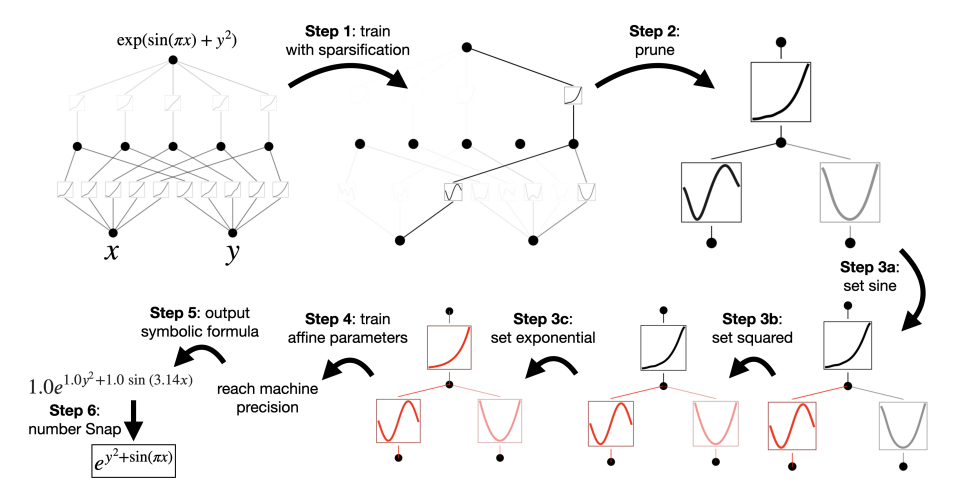
\includegraphics[width=0.85\linewidth]{LATEX//Images/advanced.png}
    \caption{Advanced KAN techniques}
    \label{fig:advanced}
\end{figure}

\subsubsection{Sparsification (Regularization)}
For MLPs, regularization, particularly L1 regularization of linear weights, is used to promote sparsity, thereby improving predictions. KANs can adopt this high-level concept, but two modifications are necessary:

\begin{enumerate}
    \item Since there are no linear weights in KANs, linear weights are replaced by learnable activation functions. Therefore, the L1 norm must be redefined for these activation functions.
    \item Experimentally, we find that L1 regularization alone is insufficient for sparsifying KANs. Instead, additional entropy regularization encourages the model to use activation functions with lower complexity and fewer degrees of freedom.
\end{enumerate}

We define the L1 norm of an activation function $\phi$ as its average magnitude over its $N_p$ inputs: $|\phi|_1$.

$$|\phi|_1 \equiv \frac{1}{N_p} \sum_{s=1}^{N_p} |\phi(x^{(s)})|$$

Then for a KAN layer $\boldsymbol{\Phi}$ with $n_{in}$ inputs and $n_{out}$ outputs, we define the L1 norm of $\boldsymbol{\Phi}$ to be the sum of L1 norms of all activation functions: $\boldsymbol{|\Phi|_1}$.

$$\boldsymbol{|\Phi|_1} \equiv \sum_{i=1}^{n_{in}}\sum_{j=1}^{n_{out}}|\phi_{i,j}|_1$$

In addition, as we have stated before, we define the regularization entropy of $\boldsymbol{\Phi}$ to be $S(\boldsymbol{\Phi})$.
$$S(\boldsymbol{\Phi}) \equiv -\sum_{i=1}^{n_{in}}\sum_{j=1}^{n_{out}} \frac{|\phi_{i,j}|_1}{\boldsymbol{|\Phi|_1}}\log(\frac{|\phi_{i,j}|_1}{\boldsymbol{|\Phi|_1}})$$

The total training objective $l_{total}$ is the prediction loss $l_{pred}$ plus L1 and entropy regularization of
all KAN layers where we define $\mu_1$, $\mu_2$ are relative magnitudes usually set to $\mu_1 = \mu_2 = 1$, and $\lambda$ controls overall regularization magnitude

$$l_{total} = l_{pred} + \lambda(\mu_1\sum_{l=0}^{L-1}\boldsymbol{|\Phi_l|_1} + \mu_2\sum_{l=0}^{L-1} S(\boldsymbol{\Phi_l}))$$

\subsubsection{Pruning}
After training with the sparsification penalty, we may also want to prune the network to a smaller subnetwork. We sparsify KANs at the node level (rather than at the edge level). For each node (say the $l^{th}$ neuron in the $l^{th}$ layer), we define its incoming and outgoing scores as $ I_{l, i}$ and $ O_{l, i}$.

$$ I_{l,i} = \max_k(|\phi_{l-1,i,k}|_1), \quad O_{l,i} = \max_j(|\phi_{l+1,j,i}|_1) $$

and consider a node to be important if both incoming and outgoing scores are greater than a threshold hyperparameter $\theta = 10^{-2}$ by default. Finally, all unimportant neurons are pruned reducing the network size.

\subsubsection{Symbolification}
In some cases, after pruning, we suspect that some activation functions are very similar to symbolic functions (such as $\cos(x)$, $\tanh(x)$, $e^x$, $\ln(x)$, etc.). The goal of Symbolification is to provide an interface to set the symbolic $\phi$ to its specified symbolic form. We will see how this leads to interpretability in Section~\ref{sec:interpre}.

Practically, we include a function $fix\_symbolic(l,i,j,f)$ that can set the activation at position $(l, i, j)$ to be $f$ if they are similar. 
However, we cannot simply set the activation function to the exact symbolic formula, since its inputs and outputs may have shifts and scaling. 
Therefore, we obtain the pre-activation values $x$ and post-activation values $y$ from samples and fit affine parameters $a$, $b$, $c$, and $d$ such that $y \approx c f(a x + b) + d$. The fitting is done by iterative search for $a$ and $b$, followed by linear regression to find $c$ and $d$. 

\subsection{Interpretability}
\label{sec:interpre}
One of the biggest drawbacks of multilayer perceptrons is their lack of interpretability. On the other hand, Kolmogorov-Arnold networks are more interpretable since they learn univariate functions at all levels, which can be inspected if needed. It is relatively easy to determine the structure learned by the network using those formulas \cite{kan_intro}.

Let's consider a KAN which is learning $f(x,y)=xy$ represented by $KAN(L=2,N=[4, 2])$.

In Figure~\ref{fig:interp} inspecting the B-splines learned by KAN, we notice how the network is working.

In the first layer, both inputs $x$ and $y$ get transformed into their squares:
\begin{itemize}
    \item Activation \#1: map $x$ to $x$ $\Rightarrow \phi_{1,1}(k) = k $ 
    \item Activation \#2: map $x$ to $x^2$ $\Rightarrow \phi_{1,2}(k) = k^2$ 
    \item Activation \#3: map $y$ to $y$ $\Rightarrow \phi_{1,3}(k) = k$ 
    \item Activation \#4: map $y$ to $y^2$ $\Rightarrow \phi_{1,4}(k) = k^2$ 
\end{itemize}

In the second layer, we take the previous output and combine it as follows:
\begin{itemize}
    \item The sum of Activation \#1 and \#3, which is $(x+y)$, gets squared by activation \#5 and have $(x+y)^2$ as output then $\phi_{2,1}(k) = k^2$.

    \item The sum of Activation \#2 and \#4, which is $(x^2+y^2)$, gets negated by activation \#6 and have $-(x+y)$ as output then $\phi_{2,2}(k) = -k$.
\end{itemize}

\begin{figure}[H]
    \centering
    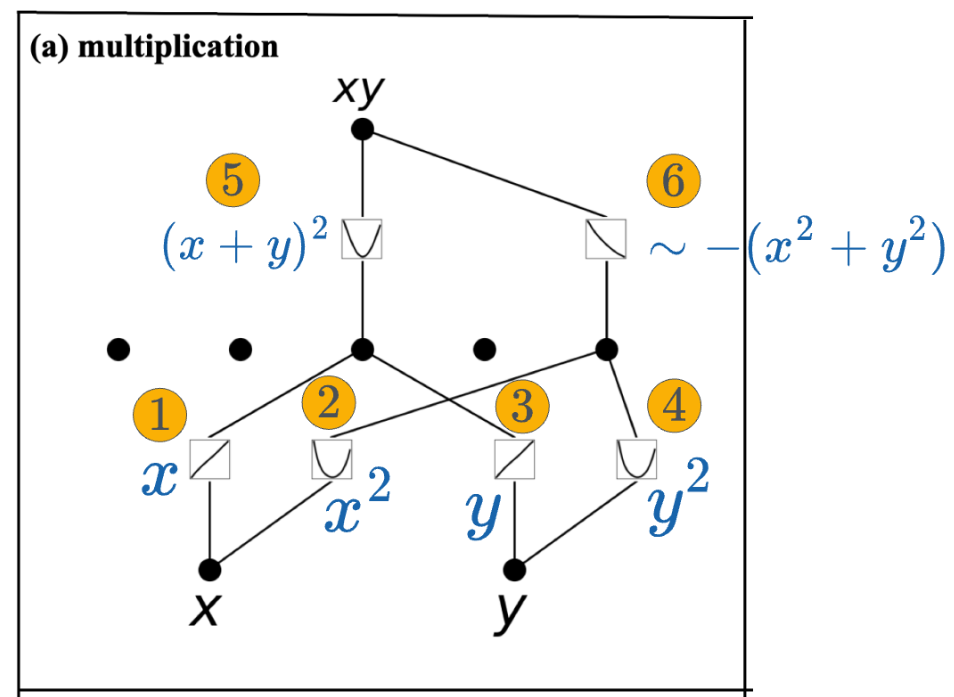
\includegraphics[width=0.5\linewidth]{LATEX//Images/interpr.png}
    \caption{Interpretation of $f(x,y)=xy$}
    \label{fig:interp}
\end{figure}

Finally, the last sum will return us $2xy$.

$$(x+y)^2 - (x^2+y^2) = x^2+y^2 +2xy - x^2 -y^2 = 2xy   $$

The interpretation is almost finished apart from the scaling factor. In the real networks the parameters $w_s$ in the last layers are assigned to $0.5$ then the last sum will return us $xy$.

$$\frac{1}{2}(x+y)^2 - \frac{1}{2}(x^2+y^2) = \frac{1}{2}x^2+\frac{1}{2}y^2 +xy - \frac{1}{2}x^2 - \frac{1}{2}y^2 = xy   $$ 

We have proved that the network can be very easy to interpret by extracting the meaning from $\phi_{i,j}(k)$.

From the Paper \cite{KAN} in Figure~\ref{fig:interp2} we will see more examples of interpretability tasks.

\begin{figure}[H]
    \centering
    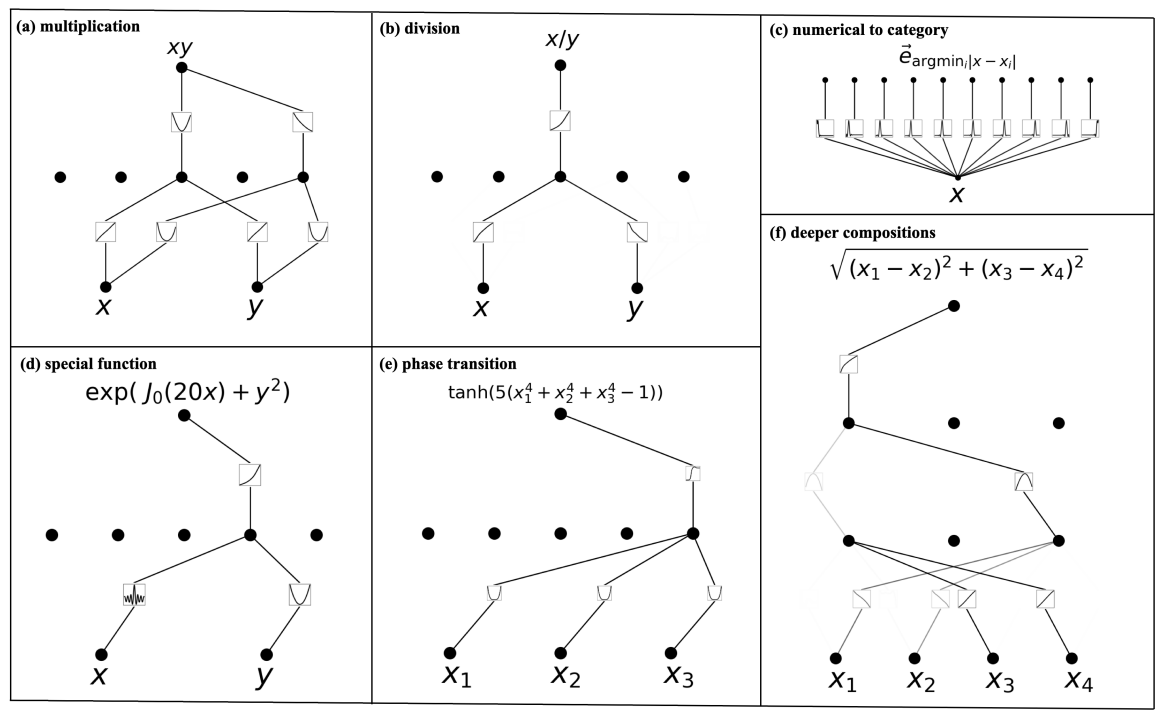
\includegraphics[width=0.8\linewidth]{LATEX//Images/interpr2.png}
    \caption{Interpretation of different functions}
    \label{fig:interp2}
\end{figure}